\section{Statistical Analysis}
Tables \ref{tab:tab1} and \ref{tab:tab2} provide an overview of the statistical properties of the \textsc{BanglaBook} dataset. The sentiment doughnut chart in Figure-\ref{fig:donut_charta} illustrates the proportion of positive, neutral, and negative reviews, while the rating doughnut chart in Figure-\ref{fig:donut_chartb} displays the percentage of reviews that correspond to each rating on a scale of 1 to 5.

\definecolor{NavyBlue}{HTML}{0066CC}
\definecolor{ForestGreen}{HTML}{228B22}
\definecolor{Lavender}{HTML}{745BB1}
\definecolor{Crimson}{HTML}{DC143C}
\definecolor{Red}{HTML}{FF0000}
\definecolor{Cyan}{HTML}{33FFFF}
\definecolor{LightGreen}{HTML}{80FF00}
\definecolor{Gold}{HTML}{CCCC00}
\definecolor{Pink}{HTML}{FF00FF}
Upon analyzing the sentiment chart, it appears that the majority of the reviews (\textcolor{NavyBlue}{124,084} + \textcolor{orange}{17,503} = 141,587 samples) are positive, with a significant portion also being negative (\textcolor{Lavender}{2,728} + \textcolor{ForestGreen}{6,946} = 9,674 samples). A relatively small fraction of the reviews are neutral (\textcolor{Crimson}{6,804} samples). This suggests that overall, the books have been well received by the readers, with the majority expressing favorable opinions. The distribution of the dataset is representative of real-world scenarios and it tessellates well with previous content analysis works on book reviews \cite{lin2005effect,sorensen2004any}. 
% In the rating chart, it is evident that the majority of the reviews have awarded the books a high rating, with a large number of 5-star (1,24,084 samples) and 4-star reviews (17,503 samples). There is a relatively small number of 1-star (6,946 samples) and 2-star (2,728 samples) reviews, indicating that the books have received mostly positive ratings.
In Figure-\ref{fig:categorywise}, we can visualize an illustration of the sentiment distribution among the 5 most frequently reviewed categories of books. We can gain some salient insights from the popularity of these genres. Contemporary novels are bestsellers as they reflect current events, social issues, and trends, making them relatable and thought-provoking for the readers while self-help and religious books provide guidance, inspiration, and a sense of purpose, catering to individuals' quest for personal growth and spiritual fulfillment.

\begin{figure}[h]
    \centering
    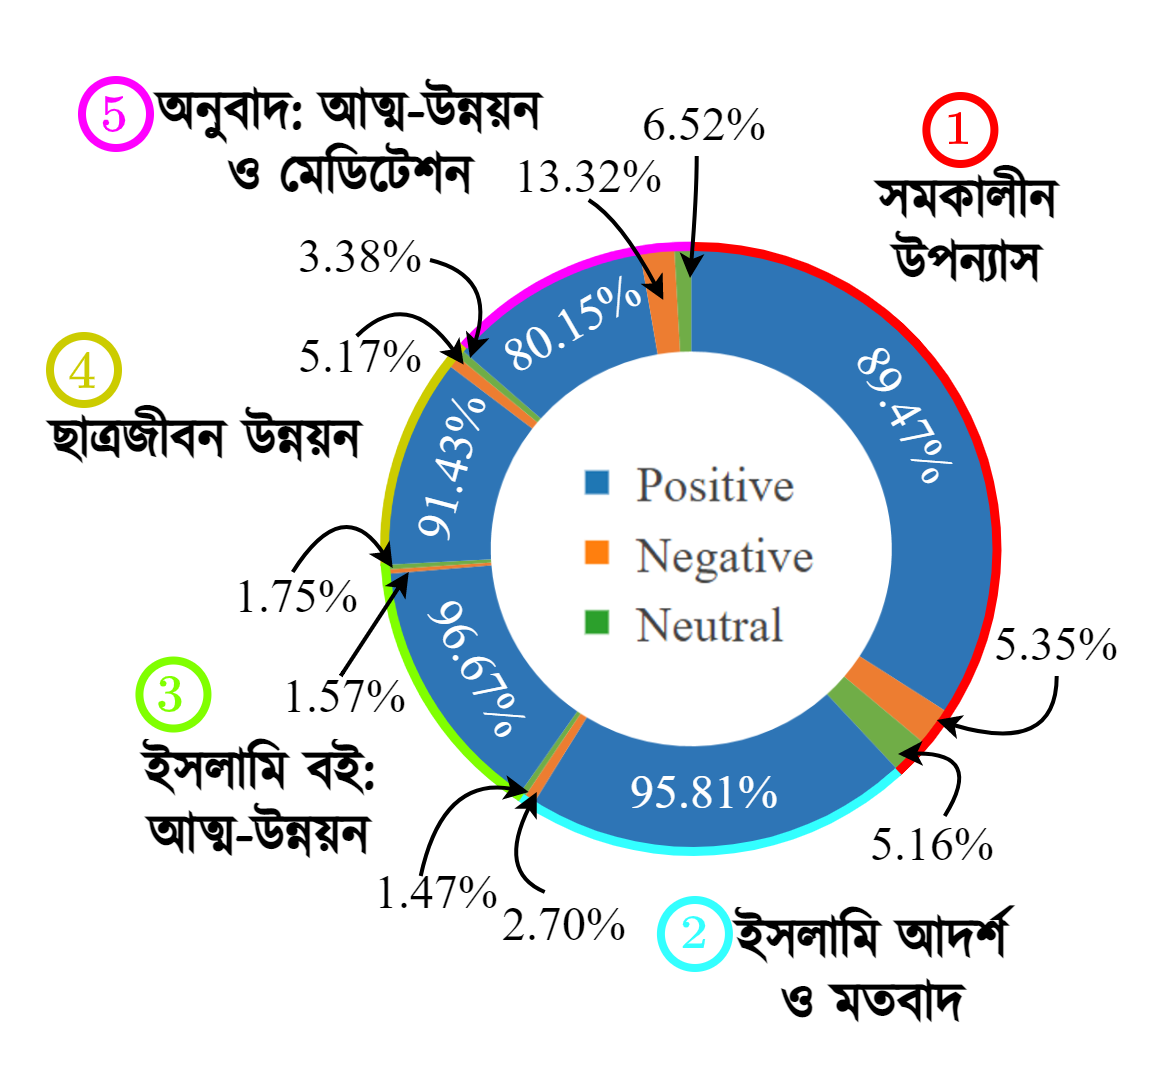
\includegraphics[scale=0.19]{images/ACLBookReview8.PNG}
    \caption{$\text{Sentiment}\hspace{2.5pt}\text{Distribution}\hspace{2.5pt}\text{of}\hspace{2.5pt}\text{top}\hspace{2.5pt}\text{5}\hspace{2.5pt}\text{most}\hspace{2.5pt}\text{popular}$$\\$genres.$\hspace{2.5pt}$In$\hspace{2.5pt}$clockwise$\hspace{2.5pt}$order,$\hspace{2.5pt}$\bangla  \textcolor{Red}{সমকালীন}$\hspace{2pt}$\textcolor{Red}{উপন্যাস}$\hspace{2pt}$$\text{(Contemp-}\\\text{orary}$$\hspace{2.5pt}$$\text{Novel)}$,$\hspace{2pt}$\bangla \textcolor{Cyan}{ইসলামি}$\hspace{2pt}$\textcolor{Cyan}{আদর্শ}$\hspace{2pt}$\textcolor{Cyan}{ও}$\hspace{2pt}$\textcolor{Cyan}{মতবাদ}$\hspace{2pt}$$\text{(Islamic}\hspace{2.5pt}\text{Ideals} \hspace{2.5pt}\text{and}$$\\$$\text{Doctrines),}$$\hspace{2pt}$\bangla \textcolor{LightGreen}{ইসলামি}$\hspace{2.5pt}$\textcolor{LightGreen}{বই:}$\hspace{2.5pt}$\textcolor{LightGreen}{আত্ম}$\hspace{2.5pt}$\textcolor{LightGreen}{উন্নয়ন}$\hspace{2.5pt}$$\text{(Islamic}\hspace{2.5pt}\text{Books:}\hspace{2.5pt}\text{Self-}\\\text{Development)}$,$\hspace{2.5pt}$\bangla \textcolor{Gold}{ছাত্রজীবন}$\hspace{2.5pt}$\textcolor{Gold}{উন্নয়ন}$\hspace{2.5pt}$$\text{(Student}\hspace{2.5pt}\text{Life}\hspace{2.5pt}\text{Developm-}\\\text{ent)}$,$\hspace{2.5pt}$\bangla \textcolor{Pink}{অনুবাদ:}$\hspace{2.5pt}$\textcolor{Pink}{আত্ম-উন্নয়ন}$\hspace{2.5pt}$\textcolor{Pink}{ও}$\hspace{2.5pt}$\textcolor{Pink}{মেডিটেশন}$\hspace{2.5pt}$$\text{(Translated}\hspace{2.5pt}\text{Books:}\\\text{Self-Development}$$\hspace{2pt}$$\text{and}\hspace{2.5pt}\text{Meditation).}$}
    \label{fig:categorywise}
\end{figure}
% \begin{figure}[h]
%     \centering
%     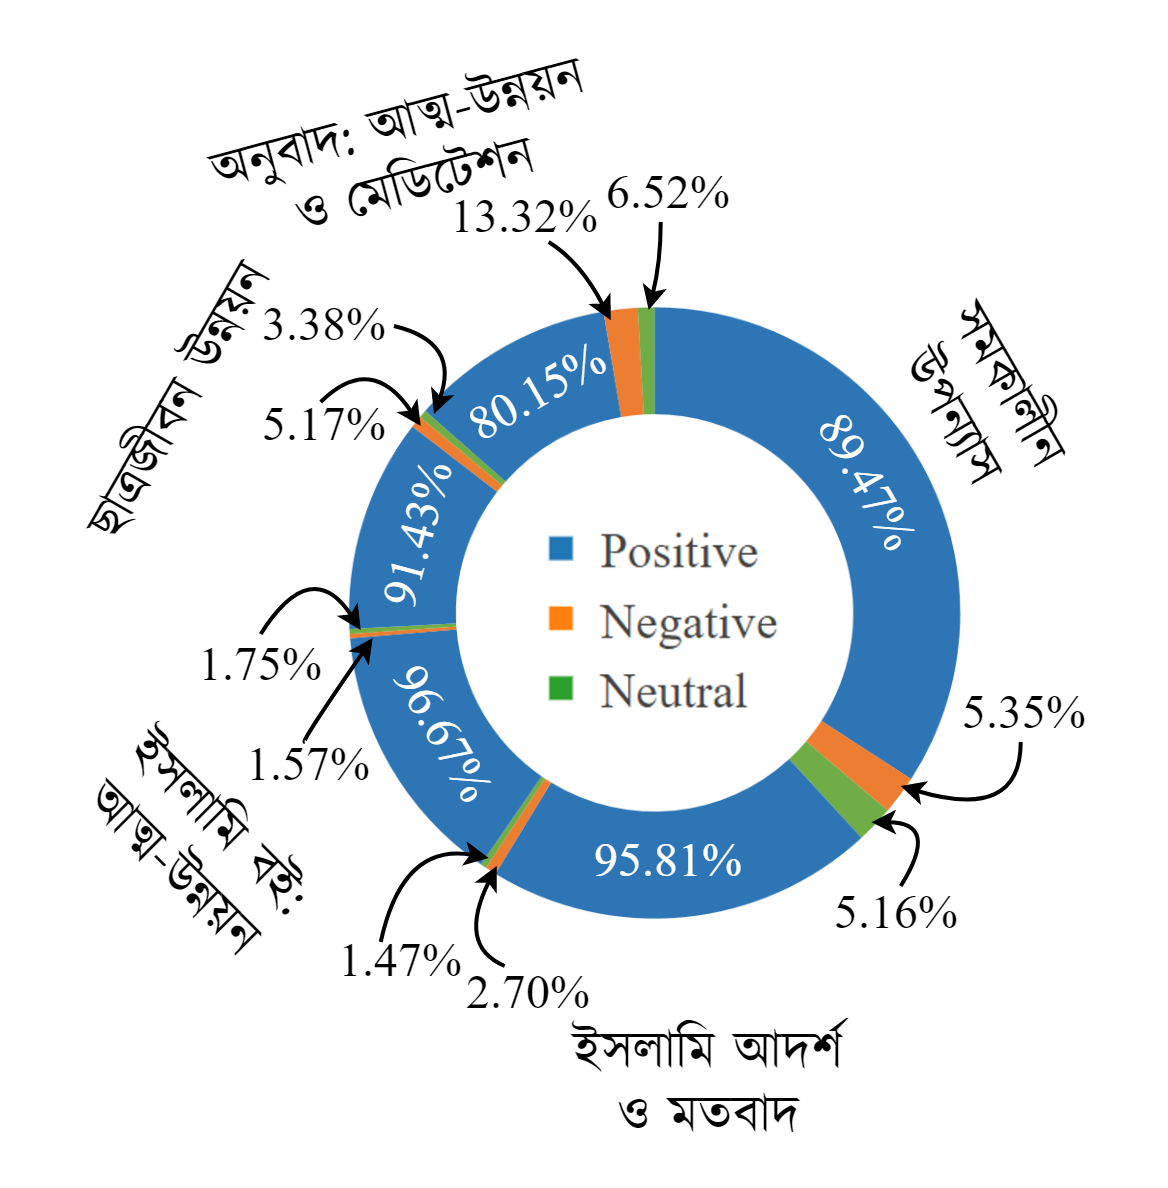
\includegraphics[scale=0.13]{images/ACLBookReview6.PNG}
%     \caption{Sentiment Distribution of top 5 most popular genres. In clockwise order, \bangla সমকালীন উপন্যাস $\text{(Contemporary Novel)}$, \bangla ইসলামি আদর্শ ও মতবাদ $\text{(Islamic Ideals and Doctrines)}$, \bangla ইসলামি বই: আত্ম-উন্নয়ন $\text{(Islamic Books: Self-Development)}$, \bangla ছাত্রজীবন উন্নয়ন $\text{(Student Life Development)}$, \bangla অনুবাদ: আত্ম-উন্নয়ন ও মেডিটেশন $\text{(Translated Books: Self-Development and Meditation)}$}
%     \label{fig:categorywise}
% \end{figure}

